\documentclass[a5paper]{article}

\usepackage{amsmath, amssymb}
\usepackage{multicol}
\setlength{\columnsep}{1cm}
\usepackage[margin=0.75in]{geometry}
\usepackage{graphicx}
\graphicspath{ {../../../Images/COIT11240/} }
\usepackage[breaklinks, hidelinks]{hyperref}
\usepackage{siunitx}
\usepackage{tikz}
\usetikzlibrary{patterns, positioning, arrows.meta}
\usepackage[american]{circuitikz}
\usepackage{pgfplots}
\pgfplotsset{compat=newest}
\usepgfplotslibrary{external}
\usepackage{stix}
\usepackage{ragged2e}
\usepackage{enumitem}
\usepackage{polynom}

\newcommand{\minus}{\scalebox{0.5}[1.0]{$-$}}
\newcommand{\sech}{\mathrm{sech}}
\newcommand{\csch}{\mathrm{csch}}
\setcounter{secnumdepth}{4}
\renewcommand\paragraph{\@startsection{paragraph}{4}{\z@}%
% display heading, like subsubsection
                                     {-3.25ex\@plus -1ex \@minus -.2ex}%
                                     {1.5ex \@plus .2ex}%
                                     {\normalfont\normalsize\bfseries}}
\sisetup{
	round-mode = places,
	round-precision = 2,
}

\date{24\textsuperscript{th} of September 2026}

\begin{document}
	\begin{titlepage}
		\centering
		{\Huge \textsc{COIT11240 - Dashboard Design}\par}
		\vspace{1cm}
		{\Large \textsc{Lecture Notes}\par}
		\vspace{2.5cm}
		\vfill
		Authored by\par
		Lachlan J. W. Wyer
		\vfill
		\makeatletter
		{\large Document Start Date: \@date \par}
		\makeatother
		{\large Latest Update: \today\par}
	\end{titlepage}
	\tableofcontents
	\pagebreak

	\raggedright

	\section{Dashboard Design}
	\subsection{Introduction:}
	Data is a crucial point within the decision making process. FOr it to actually help employees, data must be present in an effective manner.
	\subsection{Business Intelligence:}
	Business intelligence consists of theories and methods that can be applied towards meaningful descioins. Tech associated with BI allows easy transformation from row data to charts and graphs. The generated dashboards and reports provide actionable analysis. Power BI can be linked to multiple data warehouses to show a report. Shaping transforms a dataset, whereas combining connects multiple. Dashboards give opportunity for natural language search. Not available within Power BI desktop. A dashboard can be made up of multiple sub-plots.

	\section{Making Reports}
	\subsection{Visual Overviews:}
	A visual is just a graphical representation of data (e.g. Chart, Map or Graph). It simplifies the data analysis for end users. Making the data easy to understand and make accurate and effect descion making. Power BI of WYSISWYG features for OOBE. Drag and drop features for filters and page level analysis. R-scripting and python can also be used for advanced custom workflows
	\subsection{Bar Charts:}
	\subsubsection{Horizontal}
	\begin{itemize}
		\item Bad with long category labels
	\end{itemize}
	\subsubsection{Vertical}
	\begin{itemize}
		\item Useful to display negative values
		\item Able to show data chronologically
	\end{itemize}
	\subsubsection{Stacked}
	\begin{itemize}
		\item Used when a need to compare part-to-whole relationships
	\end{itemize}
	\subsubsection{100\% Stacked}
	\begin{itemize}
		\item Same as stacked, but shown as percentages
	\end{itemize}
	\subsection{Line Charts:}
	\subsubsection{Line}
	\begin{itemize}
		\item Suit to illustrate overall trends
	\end{itemize}
	\subsubsection{Stacked Area Charts}
	\begin{itemize}
		\item Showing categories contributing to a whole
		\item Whole-to-part relationships
	\end{itemize}
	\subsubsection{Combined Chart}
	\begin{itemize}
		\item Suited for trend analysis of measures of varying degrees
	\end{itemize}
	\subsubsection{Heat Map}
	\begin{itemize}
		\item Relationship between two factors
	\end{itemize}
	\subsection{Fancy Charts:}
	\subsubsection{Pie/Donut Chart}
	\begin{itemize}
		\item A circular statistical representation of data
		\item Usually shown in precentages
	\end{itemize}
	\subsubsection{Funnel Chart}
	\begin{itemize}
		\item Illustrates linear data with sequentially connected stages
	\end{itemize}
	\subsubsection{Gauge Chart}
	\begin{itemize}
		\item Data is represented in arc to show progress towards a whole
	\end{itemize}
	\subsubsection{Waterfall}
	\begin{itemize}
		\item A chart type that contains a running total (usually over time)
	\end{itemize}
	\subsubsection{Tree Maps}
	\begin{itemize}
		\item Represents data in heirarchical order
	\end{itemize}
	\subsubsection{Cards}
	\begin{itemize}
		\item Display a single value
		\item Can be done with multi-row cards
	\end{itemize}
	\subsection{Third Party Vizuals:}
	Power BI includes the ability to dislpay third party visuals. But must be done through the app store.
	\subsection{Building a Report:}
	\begin{enumerate}
		\item Import Data sources
		\item Select data sources to include, and pregare data model
		\item Establish relationships
		\item Add visuals
		\item Prepare report
		\item Otpimize for view type (Desktop vs Mobile, Screensize)
	\end{enumerate}

	\section{Dashboard Design}
	\subsection{Executive Sale Board:}
	The specific of what executive class want are the largest items, e.g.
	\begin{itemize}
		\item How are we doing this quater?
		\item How does this quater compare to last and year-on-year?
		\item Are we on track to beat last quater?
		\item Most recent transactions?
	\end{itemize}
	When designing a dashboard, understanding who is going to interact with the dashboard the most and how they will use it is important.
	\subsection{Tips:}
	Key metrics are usually left as text. For english speakers, top left is most important, with key information and should be identifiable as just a glance. Small details are required throughout. Use good colours, that make sense together. Empahsise at particulare points with bold colours. Construct filters around the most common end-users.
	\subsection{Data Anlysis Expressions (DAX):}
	DAX is a minimal programming language for basic data calculation.
	\subsection{Calculated Columns:}
	This generates a new column within the dataset.
	\subsection{Measures:}
	Filters within Power BI that dynamically update data within the Power BI dashboards.
	\subsection{DAX Capabilities:}
	\begin{itemize}
		\item DAX expression can accept tables and columns as a reference
		\item DAX operations apply to the entire column of data
		\item DAX can take up to 64 nested functions in one expression
	\end{itemize}

	\section{DAX}
	\subsection{What is DAX?:}
	DAX is a collection of function, expressions and constants. DAX helps create information from data already in the model.
	\subsection{Functions:}
	There are pre-defined formulas that perform calculations by using specific values. The arguements can be other functions, formula, column references or logic values.
	\subsection{Time Intelligence Formulas:}
	These are functions that define or select date ranges and perform dynamic calculations based on them.

	\section{Accessing Databases in Power BI}
	\subsection{Access Databases:}
	A Microsoft DBMS that combines MS Jet DB engine with a GUI and SDKs. MS Access stores information in DBs, using the following steps:
	\begin{itemize}
		\item Create the DB
		\item Data Input
		\item Query
		\item Report
	\end{itemize}
	\subsection{Data Definition:}
	Within Access rows can be defined to ensure data integrity. Such as, Only date fields can be stored in DOB column.
	\subsection{Data Control:}
	Spread sheets are good for single user problems. However problems occur when multiple users wish to have access.
	\pagebreak
	\subsection{Objects:}
	MS Access use object to aid listing and organizing of informaiton:
	\begin{itemize}
		\item Queries
		\item Forms
		\item Reports
		\item Table
	\end{itemize}
	\subsubsection{Table}
	The table is an object that is used to define and store data. Each field must have a unique name and data type. PK and FK uniqueness constraints.
	\subsubsection{Query}
	A query is an object that provides a custom view of data from at least 1 table. MS Access queries can be done through a GUI or SQL.
	\subsubsection{Report}
	A report is an object in desktop DBs designed for printing, formatting, calculating, and summarizing selected data.

	\section{Gateways}
	\subsection{External Tools:}
	External tools can be used within Power BI to extend its functionality beyond normal. Most external tools are not and should not be trusted without proper verifiction. One of the popular ones is conditional formatting on graphs.
	\subsection{Choosing the Right Vizualisation:}
	The simplest chart which conveys the correct meaning is the correct chart. Common charts to avoid are 3D graphs, pie (or pie like charts) when not comparing percentages. Best practice is to be consistent with chart scale on axes, chart dimension ordering and colours for values. Remove unnessary clutter that is not needed in the chart.
	\subsection{Gateways:}
	Gateways are used to connect on premised DBs and dynamically update the pages within Power BI. It does this through a proxy connection to Azure.

	\section{Power BI Pro}
	\subsection{Why Pro?:}
	Power BI Pro is required to collaborate and RTE sharing of the Power BI dashboard.
	\subsection{Work Spaces:}
	These are containers for dashboards, reports, workbooks, datasets and dataflows within Power BI.
	\subsection{Dataflows:}
	A dataflow help organization to unify data from multiple datasources (ETL). An optional process but useful with large and/or complex projects.
	\subsection{Datasets:}
	A dataset is simply a collection of data that can be imported or connected to Power BI. Datasets are associated with workspaces and a single dataset can be apart of many workspaces.
	\subsection{Reports:}
	A Power BI report is one or more pages of vizualizations. All visualizations in a report came from one dataset. One report:
	\begin{itemize}
		\item Is contained to a single workspace
		\item Can be associated with at least one dashboard
		\item Created from one dataset
	\end{itemize}
	\subsection{Dashboard:}
	This is something that is created in Power BI service. It is a single canvas with at least one widget.

	\section{Reports from SQL}
	\subsection{Importing SQL Data:}
	Import Mode - Used in the import screen. This data is cached on the machine. For up-to-date data the used will to refresh the dataset.\\
	Direct Query Mode - Direct Query does not import the data into Power BI rather is it a direct connection between the data base and Power BI. As such data within can be considered real-time.
	\begin{center}
		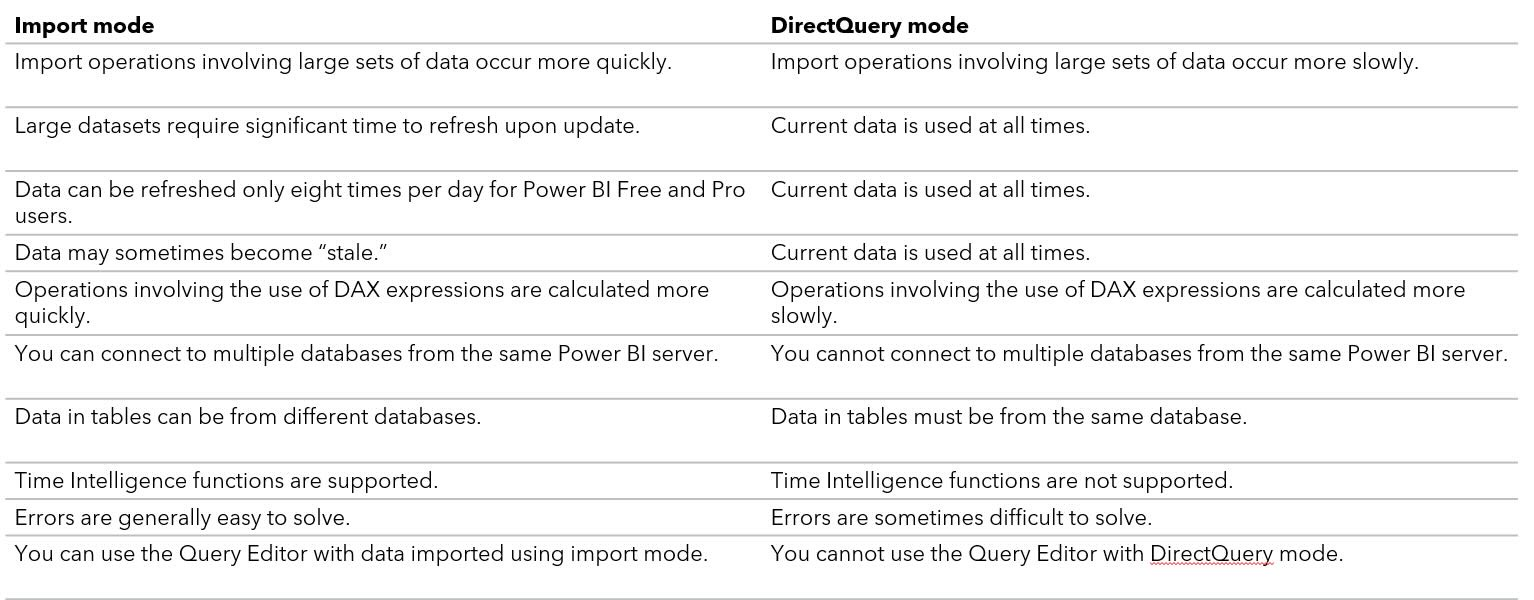
\includegraphics[scale=0.25]{direct-query.png}
	\end{center}
	\subsection{Data Gateway:}
	A gateway can be used to create a secure connection between the SQL DB and Power BI. Similar to the Direct Query Mode, Gateways can be configured to refresh at specific times.
	\subsection{Row Level Security:}
	When reports are published all the Power BI users have access to the tables and fields. As well as the data within the cells. RLS achieves this by limiting the rows a person see and modify within a report.\\
	Limitations of RLS is that the row rules must be defined within the Power BI desktop. It cannot be simply done through the Power BI service
\end{document}
